\chapter{How Bitcoin Works}

\begin{summary}
The prologue of this chapter briefly explains the rationale behind writing this book. What follows is The rest of the chapter is a high-level introduction of how Bitcoin works that acts as a summary of things that the reader must know about before moving into the following chapters. The operation of the Bitcoin network is demonstrated with a walkthrough of a transaction and its journey from its creation up until its final destination, the Bitcoin blockchain.
\end{summary}

\section{Prologue}
This book is not about introducting what Bitcoin is. The readers are expected to understand the basics of the peer-to-peer network, what addresses and private keys are as well as have some experience using wallets and sending bitcoins\footnote{When we refer to the coins we will use \emph{bitcoin(s)} (lowercase `b') and when we refer to the protocol or the network we will use \emph{Bitcoin} (uppercase `B')}. The aim of this book is to help people delve deeper and in particular learn how to \emph{talk} to the Bitcoin network programmatically.

I started teaching Bitcoin programming in 2016. I have given hundreds of presentations in meetups or seminars and from 2017 higher education courses. Every year I was improving and updating my material to keep it as relevant as possible. Luckily, Bitcoin progresses at a steady pace while always keeping backwards compatibility. This is convenient because existing material will always be valid even though better alternatives might be introduced in the future.
  
To understand the material better myself and to improve the material in my courses I started an open source Python library, called bitcoin-utils\footnote{https://github.com/karask/python-bitcoin-utils}. The library was created for educational purposes and not for computational efficiency and that might be evident in certain parts of the implementation. Before starting this library I had investigated several other well-known Python libraries but I did not find an appropriate one for educational purposes. Some were too low-level with limited documentation while others where abstracting concepts that I deemed where important for students to understand.

This book is about teaching Bitcoin programming. Throughout the years I have prepared a lot of material based on my early code experiments, the bitcoin-utils library and several online resources, especially the Bitcoin Stack Exchange\footnote{https://bitcoin.stackexchange.com/} and the excellent Bitcoin Book\footnote{https://github.com/bitcoinbook/bitcoinbook} by A. Antonopoulos. While I try to always credit the initial sources that I have consulted over the years it is very possible that I have missed some. Please let me know and I will update accordingly.

My hope is that this book consolidates all this teaching material with practical examples so as to help others understand Bitcoin programming. 

I have been using a Linux-based machine and thus most command-line examples are from \pyth{bash} shell. However, people comfortable with other Operating Systems should have no issues to adjust as needed.

\section{The Story of a Transaction}
Transactions specify the transfer of bitcoin ownership. Assume we have three actors; Zed, Alice and Bob. Zed has sent 1.5 bitcoins to Alice with $TX_x$ and Alice wants to send 1 bitcoin to Bob. The transaction history will already have an entry of how Alice got her bitcoins (e.g. from Zed).

\begin{remark}
Internally, the Bitcoin protocol operates with satoshis: $1~satoshi = 0.00000001~BTC$. Thus, when we want to transfer 1 BTC we actually transfer $100000000~satoshis$.
\end{remark}

To send 1 bitcoin (or \emph{BTC}) Alice needs to create a transaction $TX_y$ that sends 1 BTC to Bob. We know that Alice has at least 1.5 BTC from $TX_x$.

\begin{emphbox}
\begin{lstlisting}
    $TX_x$: 1Zed transfers 1.5 BTC to 1Alice
    $TX_y$: 1Alice transfers 1 BTC to 1Bob
\end{lstlisting}
\end{emphbox}

The names 1Zed, 1Alice and 1Bob are short for the actual bitcoin addresses of Zed, Alice and Bob respectively. So Alice will send 1 BTC from her 1Alice bitcoin address to Bob to his 1Bob address.

Alice has to prove that she is indeed the owner of the address 1Alice when she creates the $TX_y$. Bob does not need to do anything to receive the bitcoins.

A transaction can consist of several \textbf{\emph{inputs}} (addresses to get bitcoins from\footnote{This is an oversimplification. In reality unspent outputs or UTXOs are used as inputs which are associated with an address.}) and several \textbf{\emph{outputs}} (addresses to send bitcoins to). When an input is used it is completely consumed; i.e. all the bitcoins that the TX contains as inputs need to be \textbf{\emph{spent}}.

\begin{figure}
\begin{center}
	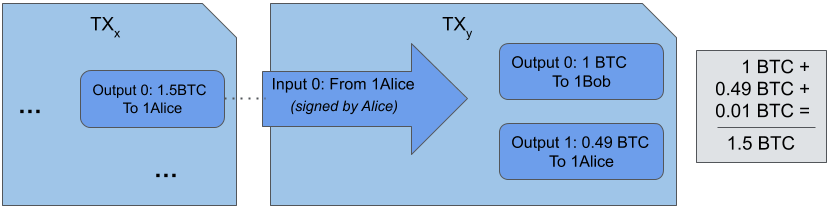
\includegraphics[scale=0.5]{images/typical-transaction}
\caption{Typical one input two outputs transaction.}
\label{fig:typical-transaction}
\end{center}
\end{figure}

The amount of all the inputs needs to be greater or equal to the amounts of outputs. If greater (recommended) the difference is an implied transaction fee that goes to the miners (see figure~\ref{fig:typical-transaction}). A typical transaction transfers some bitcoins to another user and returns the remaining bitcoins as change to the originating address or another address that the sender controls.

\begin{remark}
For privacy reasons it is recommended to send the change to a different address than the originating. Most bitcoin wallets already do this behind the scenes.
\end{remark}

Any number of inputs and outputs is possible as long as a transaction fee is included; the larger the transaction the larger the transaction fee. The unspent outputs are called \emph{Unspent Transaction Outputs (UTXOs)} and the set of UTXOs is essentially all the available bitcoins in the network.

So, for our initial example in figure~\ref{fig:typical-transaction} Alice creates $TX_y$ to send 1 BTC to Bob. What happens next?


\section{From Transactions to Blocks}
\section{Mining}
\section{Blocks and Nakamoto Consensus}
\section{Basic interaction with a node}

%problems? exercises? computer excercises???

